% Homework template for Algorithm Analysis and Design
% UPDATE: September 20, 2019 by Xu Rongchen
\documentclass[a4paper]{article}
\usepackage{ctex}
\ctexset{
proofname = \heiti{证明} %% set proof name
}
\usepackage{amsmath, amssymb, amsthm}
% amsmath: equation*, amssymb: mathbb, amsthm: proof
\usepackage{moreenum}
\usepackage{mathtools}
\usepackage{url}
\usepackage{bm}
\usepackage{enumitem}
\usepackage{graphicx}
\usepackage{subcaption}
\usepackage{booktabs} % toprule
\usepackage[mathcal]{eucal}

\usepackage{iidef} % set homework count
\usepackage{longtable}

% \usepackage[noend]{algpseudocode}
\usepackage{clrscode3e}

\thecoursename{数据仓库与数据挖掘实验报告}
\theterm{2019年秋季学期}
\hwname{第一次大作业}
\slname{\heiti{解}}
\begin{document}
\courseheader
\theusername{徐荣琛}
\thestuno{2019214518}
\theinstitute{软件学院}

\info

\begin{enumerate}
  \setlength{\itemsep}{3\parskip}
  \textbf{1.实验目的}\\
  熟悉数据仓库的建立,操作过程:\\
  (1)可能的预处理过程;\\
  (2)去噪音,去重;\\
  (3)错误修正(数据缺失,数据逻辑错误等);\\
  (4)去冗余: 数据表拆分;\\
  (5)转换成易表达的内容;\\
  仓库建立:\\
  (1)基于数据库;\\
  (2)维表,维层次和事实表的设计;\\
  基于数据立方体的数据分析。\\
  \bigskip

  \textbf{2.实验环境}\\
  实验在VirtualBox虚拟机环境下运行,硬件环境及虚拟机配置如下:\\ \medskip
  \begin{tabular}{c|c}
    \hline\hline
    处理器 & Intel(R) Core(TM) i7-8850H CPU @ 2.60GHz \\ \hline
    虚拟机内存 & 8GB\\ \hline
    虚拟机操作系统& Windows 7 Enterprise 64位\\ \hline
    数据库& Microsoft SQL Server 2008\\\hline
    分析工具& Microsoft Visual Studio 2008\\\hline
    Python环境& Python 3.7.4\\
    \hline\hline
  \end{tabular}\\
  \bigskip

  \textbf{3.实验内容}\\
  \textbf{3.1 数据清洗}\\
  \medskip
  数据清洗采用Python脚本实现。对于所有的表数据进行以下5个检查:数据类型检查、数据规约要求检查(非空、特定值检查等)
  、行内逻辑检查(如贷款金额等于期数乘每期还款数等)、表的主键唯一性检查、表间外键索引有效性检查。

  对于检查中遇到的矛盾性问题,如果解决方法比较规律且可能性单一,则采用自动处理(例如遇到无效外键引用时默认删除这条数据),
  如果可能能够实施数据修复,则脚本转入人工处理,根据人工处理结果,实施数据删除或是数据修复。

  根据最终的清洗日志,脚本一共进行了34行次的处理,一共19次外键索引有效性错误(自动修复,行删除),1次主键重复错误(行内容相同,
  自动修复,删除一行),其它出现的行内逻辑错误14次,其中修复8行次(通过近似字符串的方式或者数字数据删除意外的字符),
  删除6行次(均来自client表birth\_number逻辑错误,因存在若干个可能的修复选项而删除,例如数据“450229”,年份、月份、日期均可能发生错误)。

  具体的清洗结果如下表所示:
  \begin{center}
    \resizebox{\linewidth}{!}{ 
    \begin{tabular}{c|c|c|c|c} \hline \hline
      序& 表  & 主键值 & 错误原因 & 处理方法\\ \hline
      1&account&1675& account\_id数据类型错误&值“1675\_[typo]”更改为“1675”\\ \hline
      2&account&1801& account\_id数据类型错误&值“1801\_[I'm typo, 2]”更改为“1801”\\ \hline
      3&account&640& frequency字段不在设定值内&值“POPLATEKMESICNE”更改为“POPLATEK MESICNE”\\ \hline
      4&account&576& 存在相同行&自动删除其中一行\\ \hline
      5&card&546& type字段不在设定值内&值“golden”更改为“gold”\\ \hline
      
      6&client&2& birth\_number逻辑错误&删除行数据\\ \hline
      7&client&697& birth\_number逻辑错误&删除行数据\\ \hline
      8&client&828& birth\_number逻辑错误&删除行数据\\ \hline
      9&client&2154& birth\_number逻辑错误&删除行数据\\ \hline
      10&client&4484& birth\_number逻辑错误&删除行数据\\ \hline

      11&client&4485& birth\_number逻辑错误&删除行数据\\ \hline
      12&trans&757581& balance数据类型错误&值“15d986”更改为“15986”\\ \hline
      13&loan&5997& duration不为12的倍数&值“22”更改为“24”\\ \hline
      14&loan&5495& duration范围错误&值“-60”更改为“60”\\ \hline
      15&loan&7130& amount值不等于期数乘每期值&值“123402”更改为“123408”\\ \hline

      16&disp&2& client\_id无效外键引用&自动删除行数据\\ \hline
      17&disp&697& client\_id无效外键引用&自动删除行数据\\ \hline
      18&disp&828& client\_id无效外键引用&自动删除行数据\\ \hline
      19&disp&2154& client\_id无效外键引用&自动删除行数据\\ \hline
      20&disp&4484& client\_id无效外键引用&自动删除行数据\\ \hline

      21&disp&4485& client\_id无效外键引用&自动删除行数据\\ \hline
      22&card&339& disp\_id无效外键引用&自动删除行数据\\ \hline
      23&order&41351& account\_id无效外键引用&自动删除行数据\\ \hline
      24&order&42946& account\_id无效外键引用&自动删除行数据\\ \hline
      25&order&44598& account\_id无效外键引用&自动删除行数据\\ \hline

      26&order&46339& account\_id无效外键引用&自动删除行数据\\ \hline
      27&trans&999799& account\_id无效外键引用&自动删除行数据\\ \hline
      28&trans&999804& account\_id无效外键引用&自动删除行数据\\ \hline
      29&trans&999807& account\_id无效外键引用&自动删除行数据\\ \hline
      30&trans&999810& account\_id无效外键引用&自动删除行数据\\ \hline

      31&trans&999815& account\_id无效外键引用&自动删除行数据\\ \hline
      32&trans&999817& account\_id无效外键引用&自动删除行数据\\ \hline
      33&trans&999835& account\_id无效外键引用&自动删除行数据\\ \hline
      34&trans&999839& account\_id无效外键引用&自动删除行数据\\ \hline\hline
    \end{tabular}
    }
  \end{center}

  \medskip
  \textbf{3.2 数据仓库结构设计}\\
  \medskip
  数据仓库采用关系型逻辑模式,采用关系模型的主要原因是给定的数据集比较适合以表的形式进行表达,且各个表之间有相对明确的键值映射逻辑
  关系(即主键外键关系)。
  
  对于表进行拆解去冗余操作(如:对地区表中的大区列从地区表之中拆出,新建大区表以及地区表到大区表的外键指向),最终得到以下的数据仓库表
  结构:
  \begin{center}
    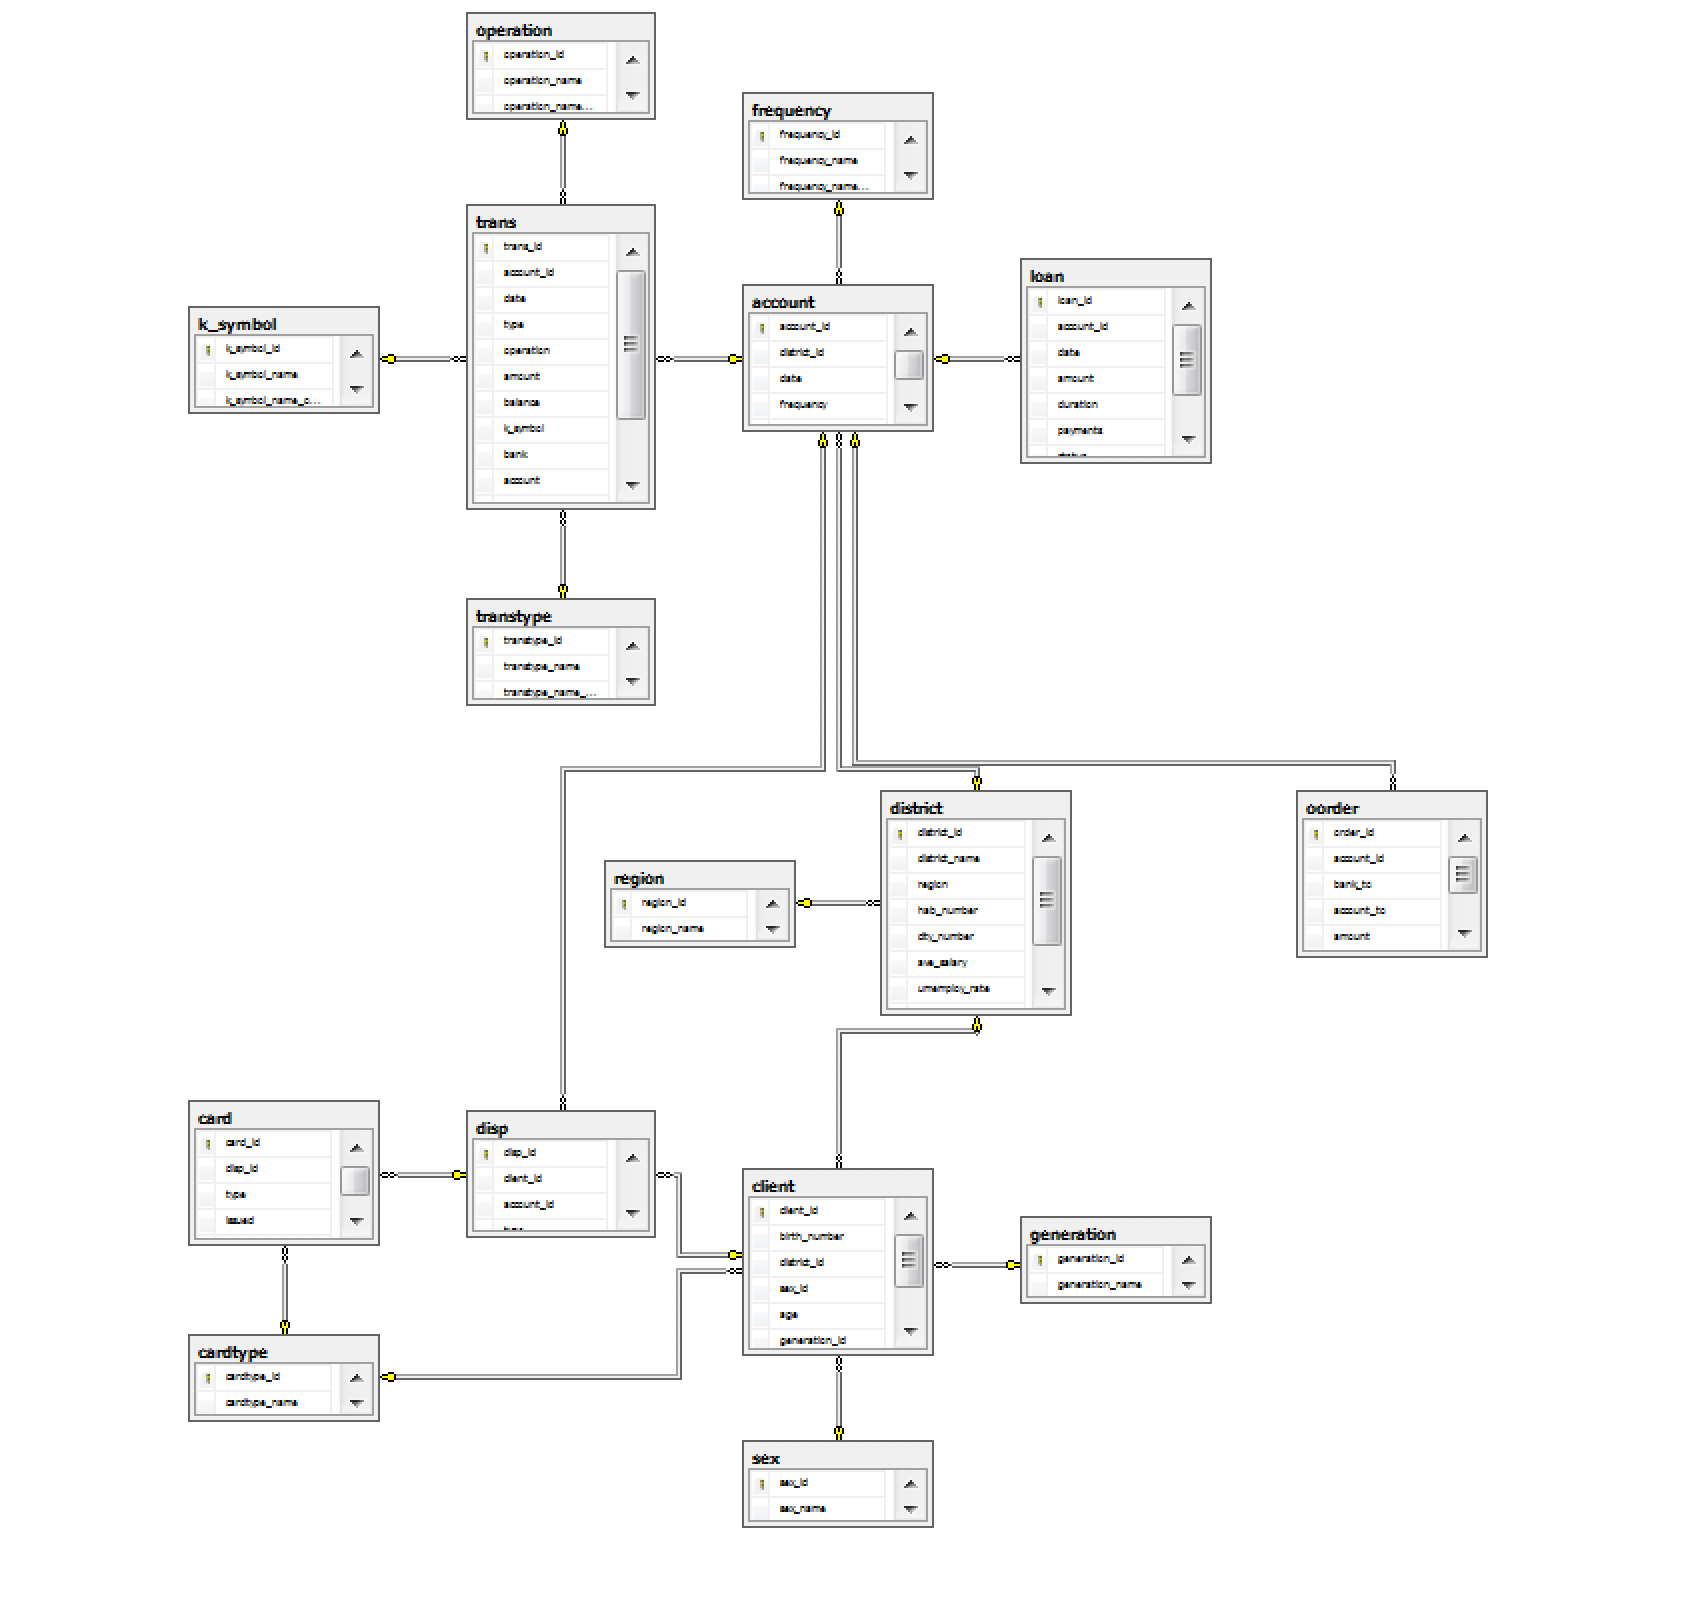
\includegraphics[scale=0.35]{Pictures/RELATION}
  \end{center}
  \medskip
  \textbf{3.3 事实表、维度表}\\
  \medskip
  根据后续的问题需要,设计必要的事实表3张,以及相关的7张维度表。

  维度表:

  (1)地区维度表(district):地区维度表由原有的地区表通过表修改得到,原有归属大区的信息转化为到大区维度表的外键;

  (2)大区维度表(region):新建表。从原有地区表的大区列字段获取所有的值。大区维度表和地区维度表构成层次结构关系;

  (3)性别维度表(sex):新建表。包括男(Male)、女(Female)两条数据;

  (4)年龄段维度表(generation):新建表。以10年为步长,分为20岁以下、20至30岁、30至40岁、40至50岁、50至60岁和60岁以上
  一共六个数据。$19X$年出生的用户的年龄定义为$99-X$;
  
  (5)信用卡类别维度表(cardtype):新建表。一共三个值,分别是junior、classic以及gold;
  
  (6)业务操作属性维度表(k\_symbol):新建表。除去主键外,包括两个字段,origin字段是从原有交易信息表(trans)以及收款服务订单信息表(order)的
  k\_symbol字段获取所有的值,为了方便数据展示,name字段是对origin字段捷克语到英语的翻译;
  
  (7)业务处理类型维度表(type):新建表。共两个值。除去主键外,包括两个字段,origin字段包括“PRIJEM”(存款)、“VYDAJ”(提款),
  为了方便数据展示,name字段是对origin字段捷克语到英语的翻译,对应“Income”和“Expenses”;

  (8)业务操作模式维度表(operation):新建表。除去主键外,包括两个字段,origin字段是从原有交易信息表(trans)的
  operation字段获取所有的值,为了方便数据展示,name字段是对origin字段捷克语到英语的翻译。
  
  事实表:

  (1)用户事实表:
  用户事实表直接由原有的用户表通过表修改得到,修改操作具体包括将原有birth\_number属性转化到年龄段和性别维度表的外键指向,并通过
  SQL查询得到所有用户最高级别的信用卡类别,并增加对于指向信用卡类别维度表的外键(如未发现有信用卡则外键为空)。用户事实表的度量值
  是行数的计数。

  用户事实表有关的关系如图:
  \begin{center}
    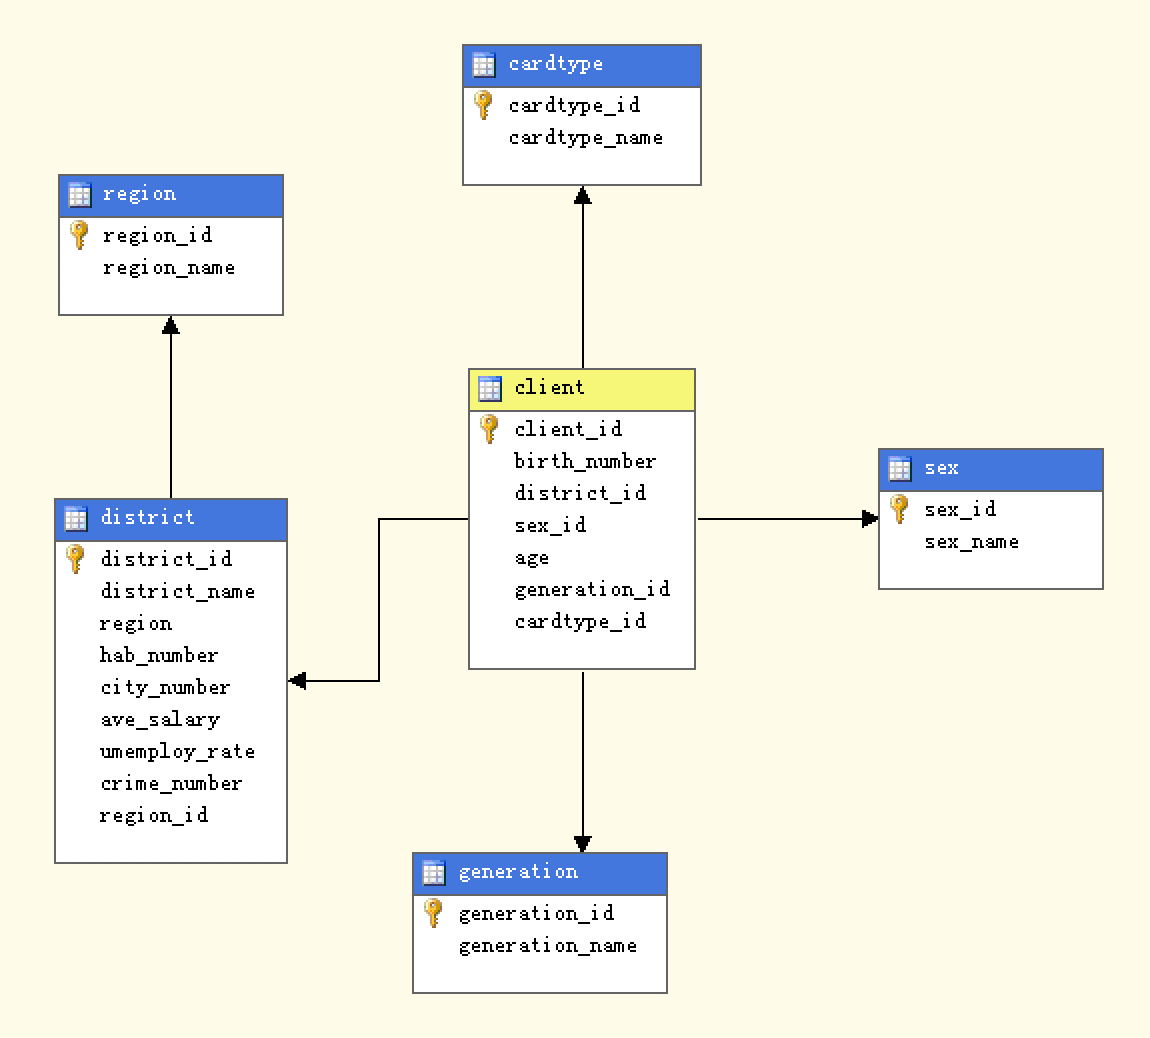
\includegraphics[scale=0.38]{Pictures/CLIENTP}
  \end{center}

  (2)交易事实表:
  为减少数据冗余,交易事实表采用视图的方式实现。通过对原有交易表(trans)、用户事实表、账户配置表(disp)的联合查询,补充所有交易
  的相关数据信息,包括交易用户的年龄段、性别、地区,交易的业务处理类型(type)、业务操作的模式(operation)、
  业务操作属性(k\_symbol)6个维度内容,对应需要建立到相应维度表的外键指向。另外,交易事实表的度量值出了行计数以外,还包括交易金额(amount)
  和交易结果(balance),以供未来的分析所需。

  交易事实表有关的关系如图:
  \begin{center}
    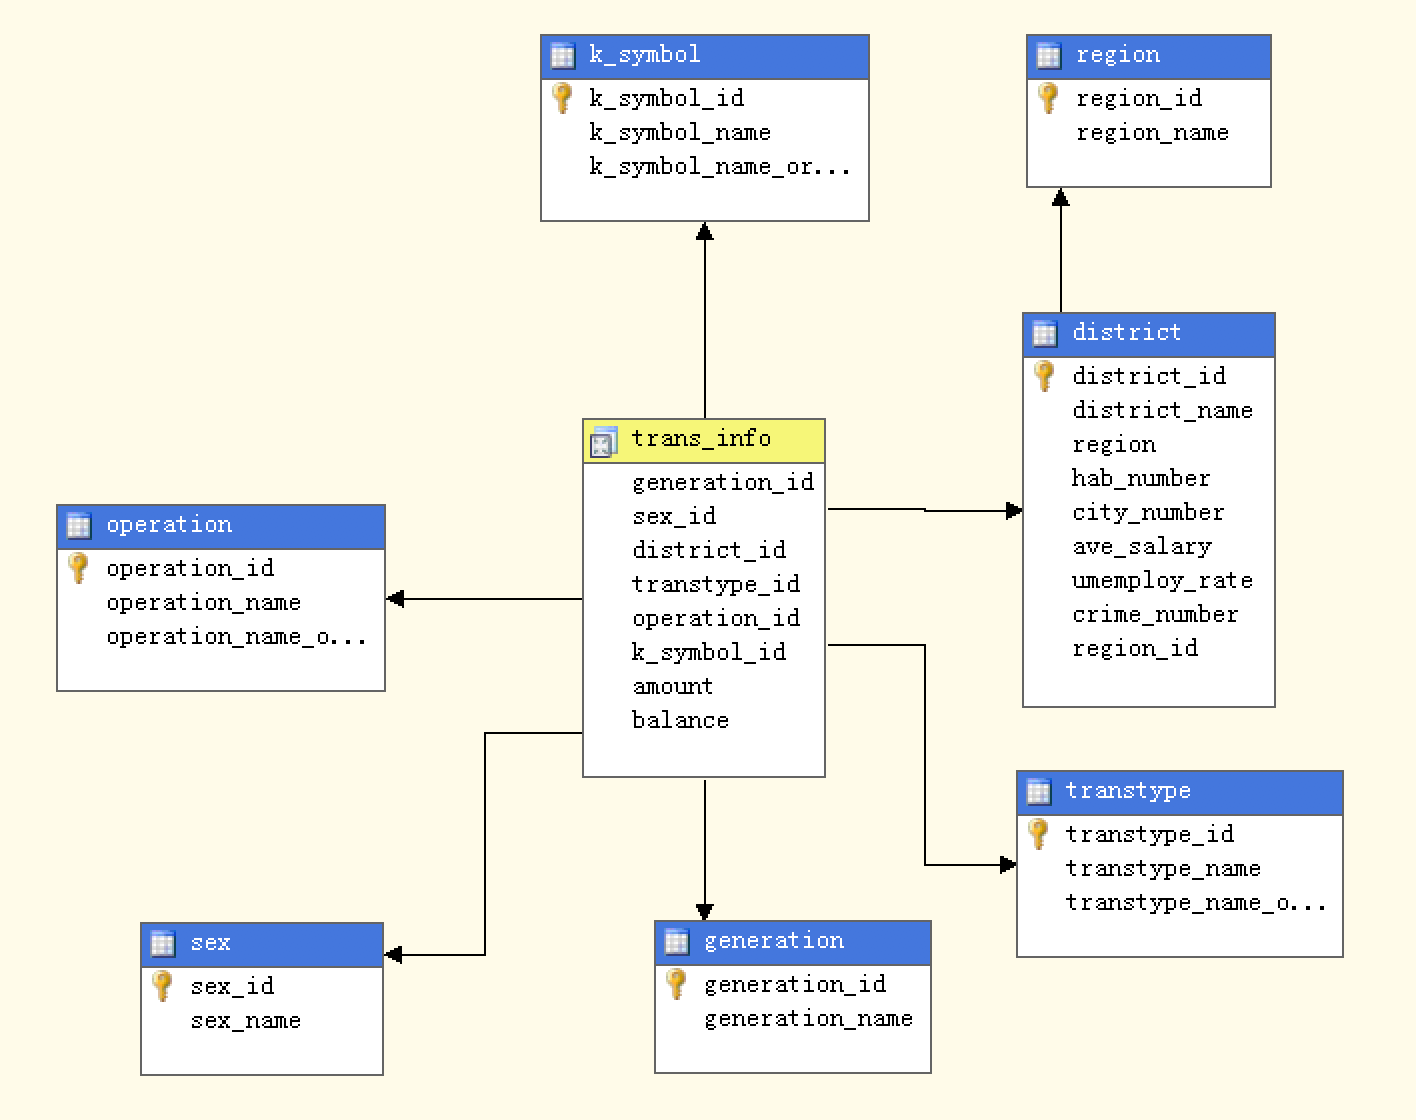
\includegraphics[scale=0.38]{Pictures/TRANSP}
  \end{center}
  
  (3)贷款用户事实表:
  为减少数据冗余,贷款用户事实表采用视图的方式实现。通过对用户事实表、贷款表(loan)、账户配置表(disp)的联合查询,筛选出所有
  在贷款记录中的涉及的用户信息。贷款用户的事实表的各个列与用户事实表保持一致。

  贷款用户事实表有关的关系如图:
  \begin{center}
    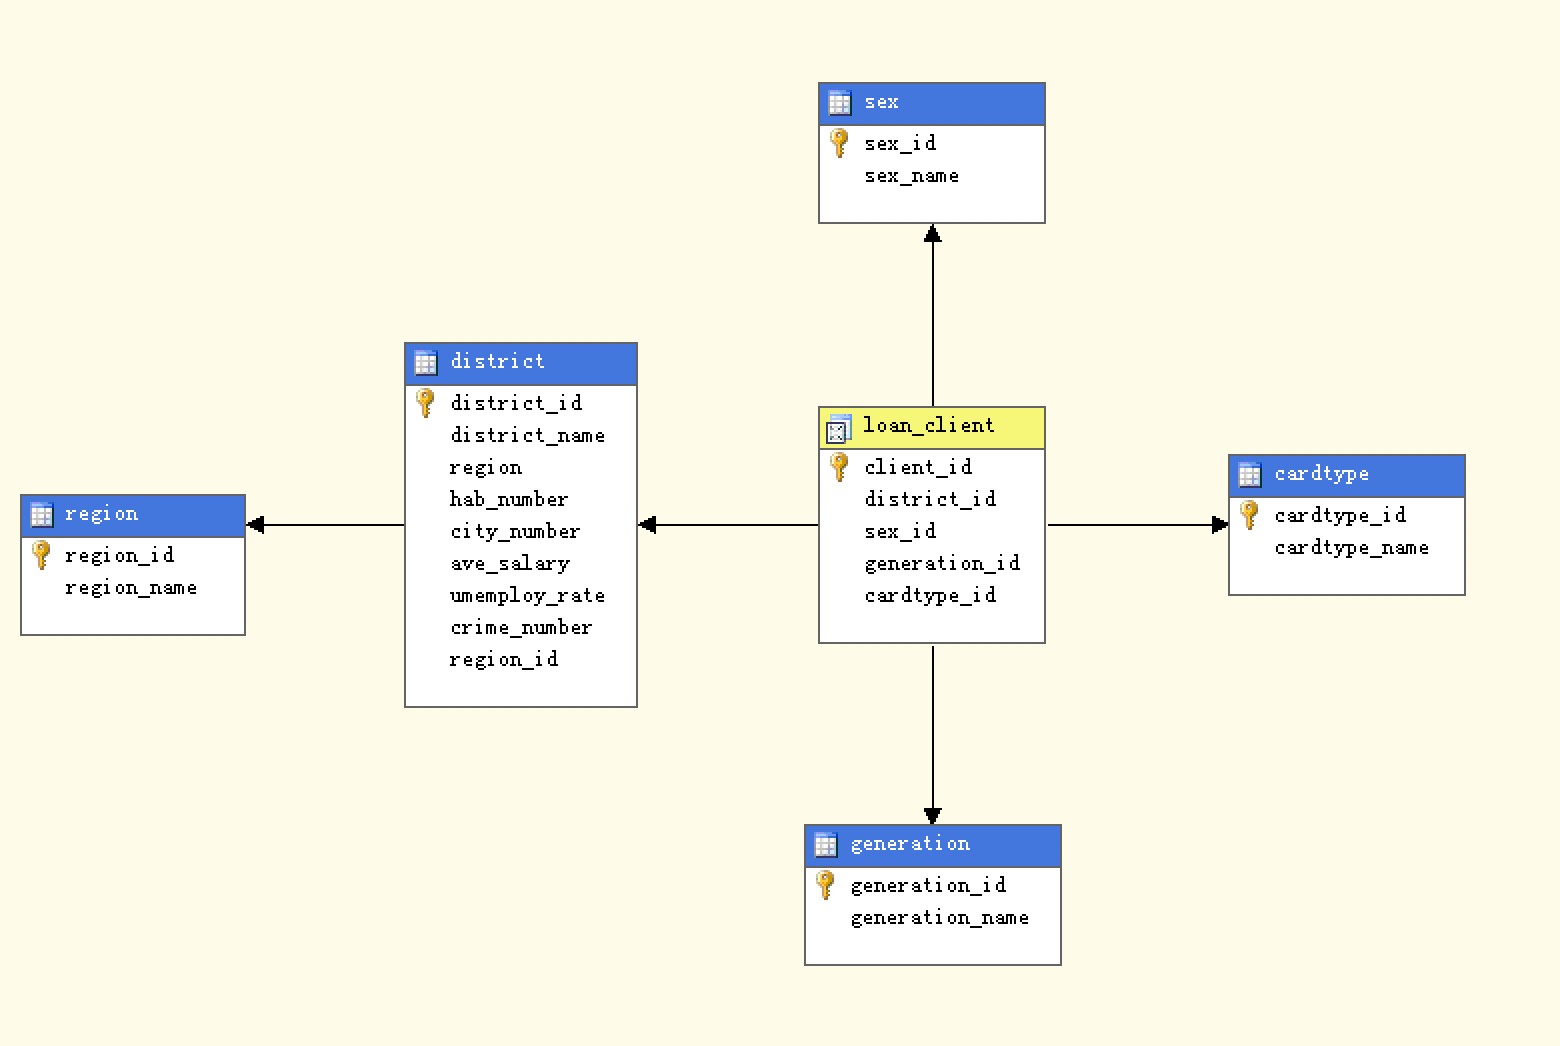
\includegraphics[scale=0.38]{Pictures/LOANP}
  \end{center}

  
  \medskip
  \textbf{3.4 基于问题的数据分析}\\
  \textbf{问题1} 针对不同性别,不同地区,不同信用卡类型(card.type)的用户,分析其中老年(年龄大于 50)用户的数量.

  \textit{1.不同性别:}对用户事实表进行筛选,性别、年龄段作为维度进行数据立方体展示,结果如图所示:
  \begin{center}
    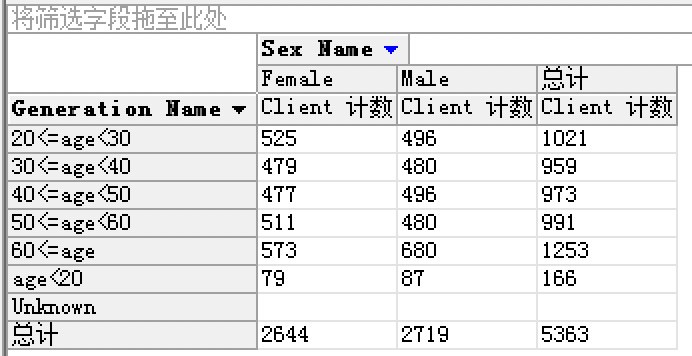
\includegraphics[scale=0.6]{Pictures/SEX}
  \end{center}
  其中,50岁以上的用户总数为2244(991+1253),其中男性1160(480+680)人,占比52\%,其中女性1084(511+573)人,
  占比48\%。

  \textit{2.不同地区:}对用户事实表进行筛选,用户地区、年龄段作为维度进行数据立方体展示,结果如图所示:
  \begin{center}
    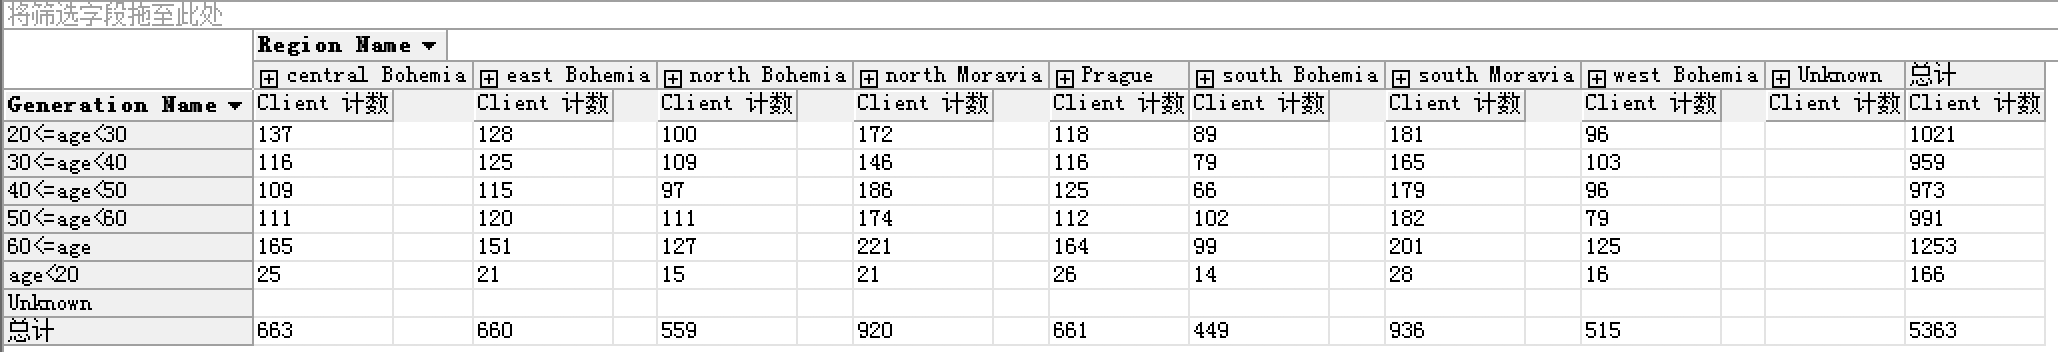
\includegraphics[scale=0.3]{Pictures/DIS}
  \end{center}
  限于篇幅,以下表格列出各个大区的50岁以上用户人数,实际如果需要更精确的地区信息,可以在大区的子项中获得。

  \begin{center}
    \begin{tabular}{c|c|c} \hline \hline
      大区名              & 60以上人数  & 占大区总人数比\\ \hline
      central Bohemia    & 276        & 42\%\\ \hline
      east Bohemia       & 271        & 41\%\\ \hline
      north Bohemia      & 238        & 43\%\\ \hline
      north Moravia      & 395        & 43\%\\ \hline
      Prague             & 276        & 42\%\\ \hline
      south Bohemia      & 201        & 45\%\\ \hline
      south Moravia      & 383        & 41\%\\ \hline
      west Bohemia       & 204        & 40\%\\  \hline \hline
    \end{tabular}
  \end{center}

  \textit{3.不同信用卡类型:}对用户事实表进行筛选,信用卡类型、年龄段作为维度进行数据立方体展示,结果如图所示:
  \begin{center}
    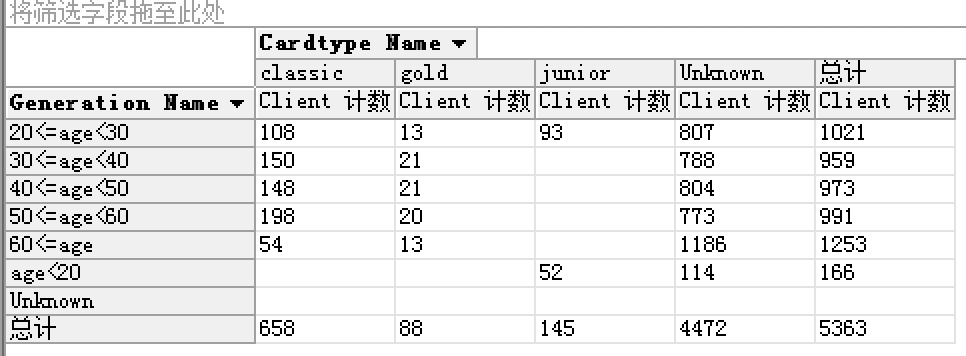
\includegraphics[scale=0.6]{Pictures/CARDTYPE}
  \end{center}
  值得注意的是,在所有的5463名客户之中,仅有891人有对应的信用卡记录,在这891人之中,junior卡145人,占比16\%,
  classic卡658人,占比74\%,gold卡88人,占比10\%。

  \textbf{问题2} 针对不同的年龄阶段,不同性别,不同地区的用户,分析交易的收入(trans.type = PRIJEM)情况,
  支出情况(trans.type = VYDAJ),净支出(所有支出减去所有收入)状况.

  \textit{1.不同年龄阶段:}对交易事实表进行筛选,年龄阶段、交易类型(收入或支出)作为维度进行数据立方体展示,结果如图所示:
  \begin{center}
    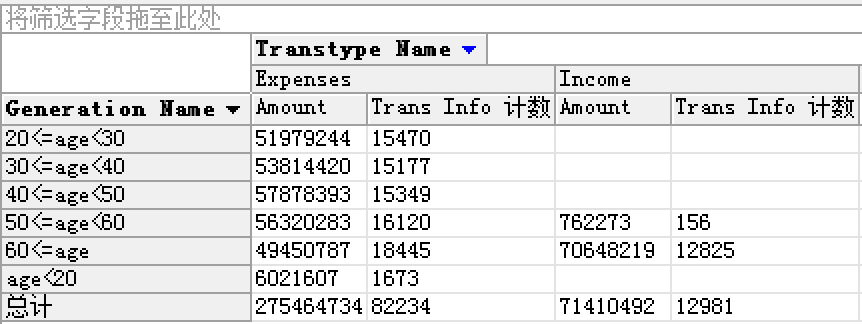
\includegraphics[scale=0.6]{Pictures/GENTR}
  \end{center}
  结果进一步计算整理的表格如下:
  \begin{center}
    \resizebox{\linewidth}{!}{ 
      \begin{tabular}{c|c|c|c|c|c|c|c} \hline \hline
        年龄段               &收入总量  & 收入次数 & 收入均值 & 支出总量  & 支出次数 & 支出均值 &总净支出 \\ \hline
        $age<20$            &        &         &         &6021607 & 1673  &3599 & 6021607\\ \hline
        $20\le age<30$      &        &         &         &51979244& 15470 &3360 & 51979244\\ \hline
        $30\le age<40$      &        &         &         &53814420& 15177 &3546 & 53814420\\ \hline
        $40\le age<50$      &        &         &         &57878393& 15349 &3771 & 57878393\\ \hline
        $50\le age<60$      &762273  &156      &4886     &56320283& 16120 &3494 & 55558010\\ \hline
        $60\le age$         &70648219&12825    &5509     &49450787& 18445 &2681 & -21197432\\ \hline\hline
      \end{tabular}
    }
  \end{center}

  \textit{2.不同性别:}对交易事实表进行筛选,性别、交易类型(收入或支出)作为维度进行数据立方体展示,结果如图所示:
  \begin{center}
    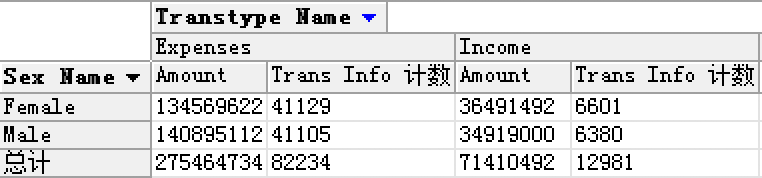
\includegraphics[scale=0.6]{Pictures/SEXTR}
  \end{center}
  结果进一步计算整理的表格如下:
  \begin{center}
    \resizebox{\linewidth}{!}{ 
      \begin{tabular}{c|c|c|c|c|c|c|c} \hline \hline
        性别          &收入总量  & 收入次数 & 收入均值 & 支出总量  & 支出次数 & 支出均值 &总净支出 \\ \hline
        Female       &36491492  &6601   &5528     &134569622 & 41129  &3272 & 98078130\\ \hline
        Male         &34919000  &6380   &5389     &140895112 & 41105  &3428 & 105976112\\ \hline\hline
      \end{tabular}
    }
  \end{center}

  \textit{3.不同地区:}对交易事实表进行筛选,用户地区、交易类型(收入或支出)作为维度进行数据立方体展示,结果如图所示:
  \begin{center}
    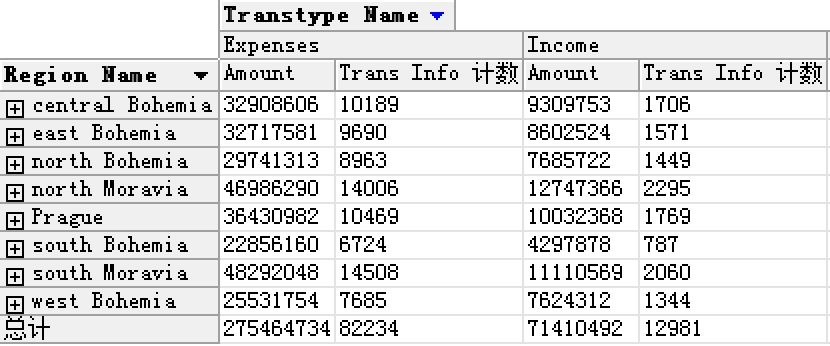
\includegraphics[scale=0.6]{Pictures/DISTR}
  \end{center}
  
  限于篇幅,以下表格列出各个大区的交易类型(收入或支出)情况,实际如果需要更精确的地区信息,可以在大区的子项中获得:
  \begin{center}
    \resizebox{\linewidth}{!}{ 
      \begin{tabular}{c|c|c|c|c|c|c|c} \hline \hline
        大区名                  &收入总量  & 收入次数 & 收入均值 & 支出总量  & 支出次数 & 支出均值 &总净支出 \\ \hline
        central Bohemia       &9309753  &1706   &5457     &32908606 & 10189  &3230 & 23598853\\ \hline
        east Bohemia          &8602524  &1571   &5476     &32717581 & 9690  &3376 & 24115057\\ \hline
        north Bohemia         &7685722  &1449   &5304     &29741313 & 8963  &3318 & 22055591\\ \hline
        north Moravia         &12747366 &2295   &5554     &46986290 & 14006  &3355 & 34238924\\ \hline
        Prague                &10032368 &1769   &5671     &36430982 & 10469  &3480 & 26398614\\ \hline
        south Bohemia         &4297878  &787    &5461     &22856160 & 6724  &3399 & 18558282\\ \hline
        south Moravia         &11110569 &2060   &5393     &48292048 & 14508  &3329 & 37181479\\ \hline
        west Bohemia          &7624312  &1344   &5673     &25531754 & 7685  &3322 & 17907442\\ \hline
        \hline
      \end{tabular}
    }
  \end{center}

  \textbf{问题3}假设你是一个银行的数据分析人员,银行希望能够放出更多的贷款。请以这个作为目标,选择合适的维度进行分析,
  告知管理人员应该把优惠政策和宣传力度集中到哪类人群。 

  从所有客户群体中筛选出所有有贷款记录的用户,首先按照用户信用卡类型和用户性别分类,建立如图所示的数据立方体:
  \begin{center}
    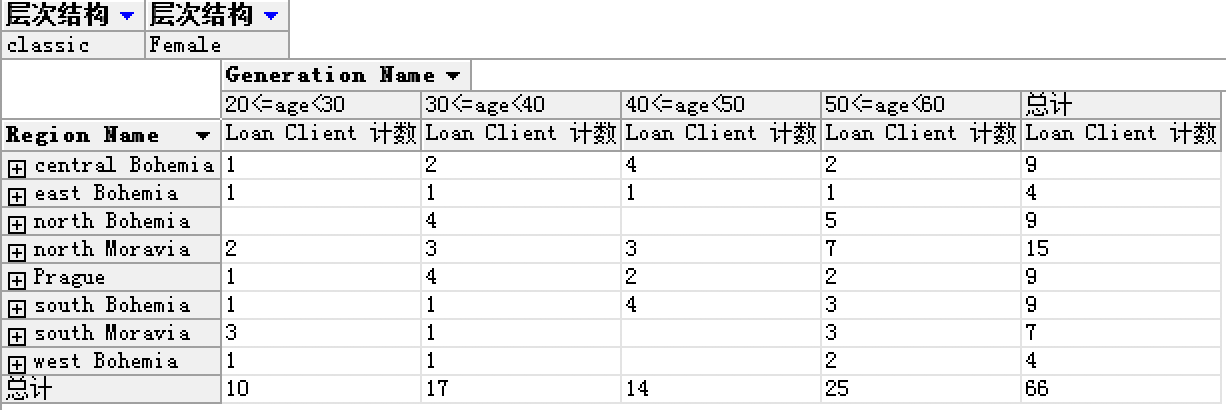
\includegraphics[scale=0.5]{Pictures/LOANINFO}
  \end{center}
  结合问题1的相关数据,可以得到以下有关卡类型、用户性别、用户年龄段、用户地区的表格:
  \begin{center}
    \begin{tabular}{c|c|c|c}\hline\hline
      卡类型 & 贷款人数 & 总人数 & 比例\\ \hline
      junior& 21& 145& 14.5\%\\ \hline
      classic& 133& 658& 20.2\%\\ \hline
      gold& 16& 88& 18.2\%\\ \hline
      unknown& 656& 4472& 14.7\%\\ \hline\hline
    \end{tabular}
  \end{center}
  从中可知,从卡类型分析,持有classic信用卡和gold信用卡的用户有更大可能性申请贷款而持有junior信用卡用户相对低。
  \begin{center}
    \begin{tabular}{c|c|c|c} \hline \hline
      性别          & 贷款人数 & 总人数 & 比例\\ \hline
      Female       &417  &2644   &15.8\%\\ \hline
      Male         &409  &2719   &15.0\%\\ \hline\hline
    \end{tabular}
  \end{center}
  从中可知,从用户性别分析,女性用户相对男性用户有略大可能性去申请贷款,但是差异不大。
  \begin{center}
    \begin{tabular}{c|c|c|c} \hline \hline
      年龄段           & 贷款人数 & 总人数 & 比例\\ \hline
      $age<20$        &21   &166   &12.7\%\\ \hline
      $20\le age<30$  &176  &1021  &17.2\%\\ \hline
      $30\le age<40$  &188  &959   &19.6\%\\ \hline
      $40\le age<50$  &186  &973   &19.1\%\\ \hline
      $50\le age<60$  &189  &991   &19.1\%\\ \hline
      $60\le age$     &66   &1253  &15.0\%\\ \hline
      \hline
    \end{tabular}
  \end{center}
  从中可以分析到年龄段在30~60岁之间段用户有更大可能性(超过19\%的可能)去申请贷款。

  分析用户地区,在所有77个地区中,发现贷款可能性与人均收入、人均犯罪事件数目强相关。

  
  在人均犯罪事件数最高的前20个地区
  (地区人均犯罪事件数高于0.0367)总计客户数目为1960,其中贷款总人次为275,占比14.0\%;而人均犯罪事件数较低的另一半地区
  (地区人均犯罪事件数低于0.0220)总计客户数目为1216,其中贷款总人次为217,占比17.8\%。因此,犯罪率低的地区则有更大的可能性
  产生贷款业务。
  
  在人均收入最低的前20个地区(低于8510),总计的客户数目为1096,其中贷款总人次为192,占比17.5\%;而在人均收入最高的前20
  个地区(高于9310),总计的客户数目为2095,其中贷款总人次为309,占比14.7\%。

  综上结论,贷款的宣传对象可以更加侧重于以下的客户群体:

  (1)持有classic或者gold类别信用卡的客户;

  (2)年龄段在30岁至60岁之间的客户;

  (3)来自低犯罪率水平地区的客户;

  (4)来自平均收入高地区的客户。
\end{enumerate}
\end{document}